% Quantum autoencoder and variational quantum anomaly detection of notebook 45b, N = 8, k = 2,
% trash = qubits 0 and 7 (TRASH[2] = (0, N-1)).
% (a) the full autoencoder: encoder U(theta) (hardware-efficient ansatz, L layers), trash qubits discarded and
%     replaced by fresh |0>, decoder U^dagger(theta); output rho_out, reconstruction fidelity F_rec.
% (b) training: only the encoder and the trash measurement are needed; the local cost
%     D_H = (1/k) sum_j <n_j> of the trash qubits is minimised with Adam at the reference ground state.
% (c) scan: the trained encoder U(theta_*) is frozen and applied to the ground state at every grid point lambda;
%     the same local cost is the anomaly score A_k(lambda | lambda_*), Eq. (8).  The decoder is never run.
\documentclass[tikz,border=6pt]{standalone}
\usepackage{amsmath,amssymb,bm}
\usetikzlibrary{arrows.meta,decorations.pathreplacing,calc,positioning,shapes.geometric}
\newcommand{\ket}[1]{\lvert #1\rangle}
\definecolor{trash}{RGB}{190,50,30}
\begin{document}
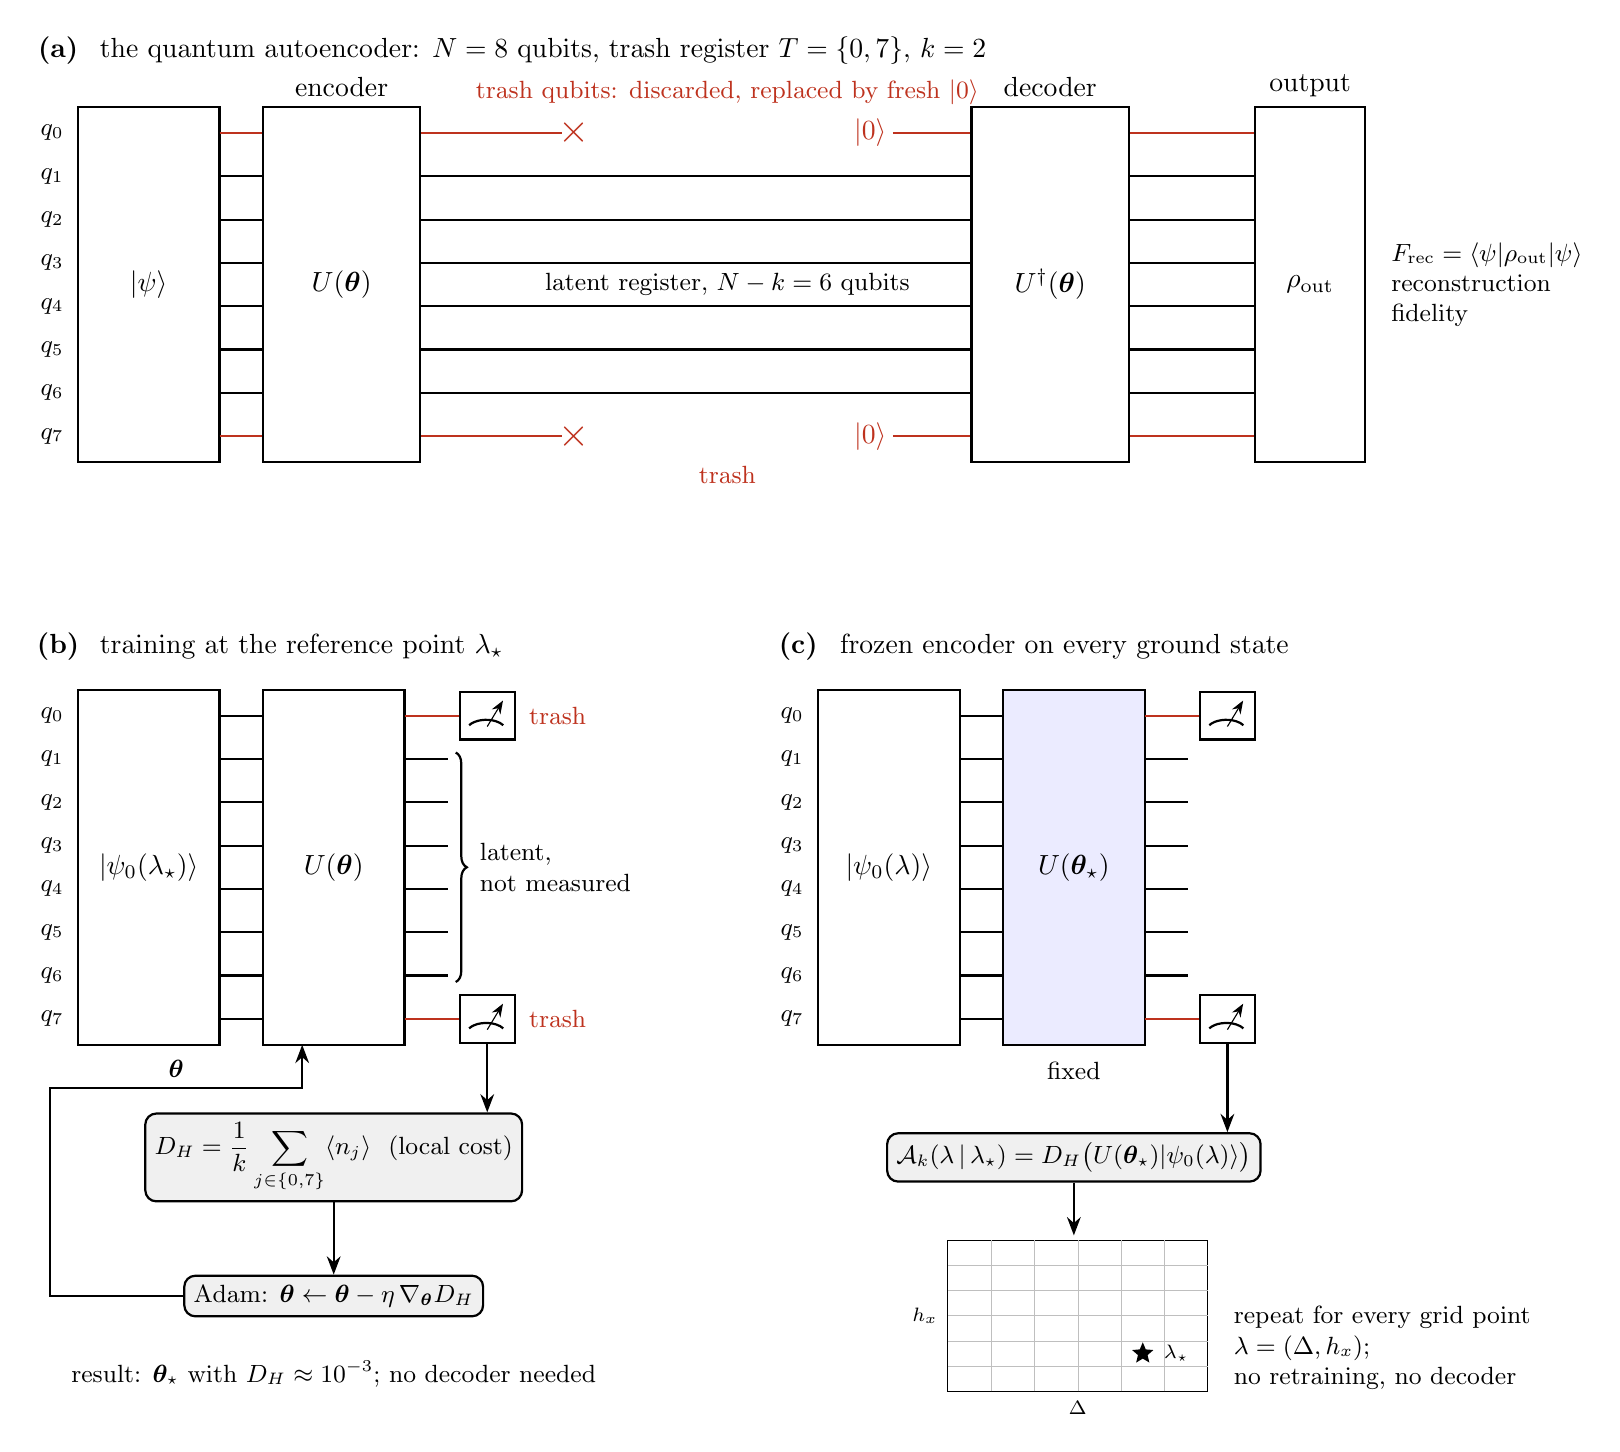
\begin{tikzpicture}[thick, >=Stealth, x=1cm, y=0.55cm]
  \newcommand{\meter}[2]{% x, y
    \draw[fill=white] (#1,#2+0.55) rectangle (#1+0.7,#2-0.55);
    \draw (#1+0.12,#2-0.22) arc (150:30:0.25);
    \draw[->, thin] (#1+0.35,#2-0.25) -- (#1+0.55,#2+0.35);}
  % ================================================================== (a) the quantum autoencoder
  \begin{scope}[yshift=7.4cm]
    \node[font=\bfseries] at (-2.2,1.9) {(a)};
    \node[anchor=west] at (-1.8,1.9) {the quantum autoencoder: $N=8$ qubits, trash register $T=\{0,7\}$, $k=2$};
    \foreach \q in {0,...,7} \node[anchor=east, font=\small] at (-2.0,-\q) {$q_{\q}$};
    \draw[fill=white] (-1.95,0.6) rectangle (-0.15,-7.6);
    \node at (-1.05,-3.5) {$\ket{\psi}$};
    \foreach \q in {1,...,6} \draw (-0.15,-\q) -- (13.0,-\q);
    \foreach \q in {0,7} { \draw[trash] (-0.15,-\q) -- (4.2,-\q); \draw[trash] (8.4,-\q) -- (13.0,-\q); }
    \draw[fill=white] (0.4,0.6) rectangle (2.4,-7.6);
    \node at (1.4,-3.5) {$U(\boldsymbol\theta)$};
    \node[above] at (1.4,0.6) {encoder};
    \foreach \q in {0,7} {
      \node[trash, font=\Large, inner sep=0pt] at (4.35,-\q) {$\times$};
      \node[trash, anchor=east] at (8.45,-\q) {$\ket{0}$};
    }
    \node[trash, font=\small, align=center] at (6.3,0.95) {trash qubits: discarded, replaced by fresh $\ket{0}$};
    \node[trash, font=\small] at (6.3,-7.9) {trash};
    \node[font=\small, fill=white, inner sep=2pt] at (6.3,-3.5) {latent register, $N-k=6$ qubits};
    \draw[fill=white] (9.4,0.6) rectangle (11.4,-7.6);
    \node at (10.4,-3.5) {$U^\dagger(\boldsymbol\theta)$};
    \node[above] at (10.4,0.6) {decoder};
    \draw[fill=white] (13.0,0.6) rectangle (14.4,-7.6);
    \node at (13.7,-3.5) {$\rho_{\rm out}$};
    \node[above] at (13.7,0.6) {output};
    \node[font=\small, anchor=west, align=left] at (14.6,-3.5) {$F_{\rm rec}=\langle\psi\vert\rho_{\rm out}\vert\psi\rangle$\\ reconstruction\\ fidelity};
  \end{scope}
  % ================================================================== (b) training
  \begin{scope}
    \node[font=\bfseries] at (-2.2,1.6) {(b)};
    \node[anchor=west] at (-1.8,1.6) {training at the reference point $\lambda_\star$};
    \foreach \q in {0,...,7} \node[anchor=east, font=\small] at (-2.0,-\q) {$q_{\q}$};
    \draw[fill=white] (-1.95,0.6) rectangle (-0.15,-7.6);
    \node at (-1.05,-3.5) {$\ket{\psi_0(\lambda_\star)}$};
    \foreach \q in {0,...,7} \draw (-0.15,-\q) -- (0.4,-\q);
    \draw[fill=white] (0.4,0.6) rectangle (2.2,-7.6);
    \node at (1.3,-3.5) {$U(\boldsymbol\theta)$};
    \foreach \q in {0,7} { \draw[trash] (2.2,-\q) -- (2.9,-\q); \meter{2.9}{-\q} }
    \foreach \q in {1,...,6} \draw (2.2,-\q) -- (2.75,-\q);
    \draw[decorate, decoration={brace, amplitude=4pt}] (2.85,-0.85) -- (2.85,-6.15)
          node[midway, right=5pt, font=\small, align=left] {latent,\\ not measured};
    \node[trash, font=\small, anchor=west] at (3.65,0) {trash};
    \node[trash, font=\small, anchor=west] at (3.65,-7) {trash};
    \node[draw, rounded corners, fill=gray!12, font=\small] (cost) at (1.3,-10.2)
         {$D_H=\dfrac1k\displaystyle\sum_{j\in\{0,7\}}\langle n_j\rangle$\ \ (local cost)};
    \node[draw, rounded corners, fill=gray!12, font=\small] (opt) at (1.3,-13.4)
         {Adam: $\boldsymbol\theta\leftarrow\boldsymbol\theta-\eta\,\nabla_{\boldsymbol\theta}D_H$};
    \draw[->] (3.25,-7.55) -- (3.25,0 |- cost.north);
    \draw[->] (cost) -- (opt);
    \draw[->] (opt.west) -- (-2.3,-13.4) -- (-2.3,-8.6) -- (0.9,-8.6) -- (0.9,-7.6);
    \node[font=\small, anchor=south] at (-0.7,-8.6) {$\boldsymbol\theta$};
    \node[font=\small] at (1.3,-15.2) {result: $\boldsymbol\theta_\star$ with $D_H\approx10^{-3}$; no decoder needed};
  \end{scope}
  % ================================================================== (c) scan
  \begin{scope}[xshift=9.4cm]
    \node[font=\bfseries] at (-2.2,1.6) {(c)};
    \node[anchor=west] at (-1.8,1.6) {frozen encoder on every ground state};
    \foreach \q in {0,...,7} \node[anchor=east, font=\small] at (-2.0,-\q) {$q_{\q}$};
    \draw[fill=white] (-1.95,0.6) rectangle (-0.15,-7.6);
    \node at (-1.05,-3.5) {$\ket{\psi_0(\lambda)}$};
    \foreach \q in {0,...,7} \draw (-0.15,-\q) -- (0.4,-\q);
    \draw[fill=blue!8] (0.4,0.6) rectangle (2.2,-7.6);
    \node at (1.3,-3.5) {$U(\boldsymbol\theta_\star)$};
    \node[font=\small] at (1.3,-8.2) {fixed};
    \foreach \q in {0,7} { \draw[trash] (2.2,-\q) -- (2.9,-\q); \meter{2.9}{-\q} }
    \foreach \q in {1,...,6} \draw (2.2,-\q) -- (2.75,-\q);
    \node[draw, rounded corners, fill=gray!12, font=\small] (score) at (1.3,-10.2)
         {$\mathcal A_k(\lambda\,|\,\lambda_\star)=D_H\bigl(U(\boldsymbol\theta_\star)\ket{\psi_0(\lambda)}\bigr)$};
    \draw[->] (3.25,-7.55) -- (3.25,0 |- score.north);
    \begin{scope}[shift={(-0.3,-15.6)}, x=0.55cm, y=0.32cm]
      \draw[thin, fill=white] (0,0) rectangle (6,6);
      \foreach \i in {1,...,5} { \draw[very thin, gray!50] (\i,0) -- (\i,6); \draw[very thin, gray!50] (0,\i) -- (6,\i); }
      \node[star, star points=5, star point ratio=2.2, fill=black, inner sep=1.3pt] at (4.5,1.5) {};
      \node[font=\scriptsize, anchor=west] at (4.75,1.5) {$\lambda_\star$};
      \node[font=\scriptsize, below] at (3,0) {$\Delta$};
      \node[font=\scriptsize, left] at (0,3) {$h_x$};
    \end{scope}
    \node[font=\small, align=left, anchor=west] at (3.2,-14.6)
         {repeat for every grid point\\ $\lambda=(\Delta,h_x)$;\\ no retraining, no decoder};
    \draw[->] (score.south) -- (1.3,-12.0);
  \end{scope}
\end{tikzpicture}
\end{document}
